% =============================================================================
% SECTION 3: METHODOLOGICAL FRAMEWORK (STREAMLINED VERSION)
% =============================================================================
% This is a more concise, equation-focused version of Section 3.
% Use this if you prefer the "4 Core Equations" structure over the detailed version.
% =============================================================================

\section{Methodological Framework}
\label{sec:methodology}

This section formalises the analytical framework underpinning the empirical analysis. The methodology integrates three complementary pillars: \textit{spatiotemporal pattern recognition} for demand characterisation, \textit{multimodal integration assessment} for first-mile/last-mile quantification, and \textit{fleet dynamics with microeconomic modelling} for operational viability evaluation. Each pillar combines established transport engineering techniques with cross-disciplinary methodological innovations.


% =============================================================================
% 3.1 SPATIOTEMPORAL PATTERN RECOGNITION
% =============================================================================

\subsection{Spatiotemporal Pattern Recognition: The Physics of Flow}
\label{subsec:spatiotemporal}

The first analytical pillar characterises the fundamental ``physics'' of e-scooter demand: where trips originate, where they terminate, and how flow intensity decays with distance.

\subsubsection{Origin-Destination Matrix Construction}
\label{subsubsec:od_construction}

The spatial structure of demand is encoded in an \textbf{Origin-Destination (O-D) matrix} $\mathbf{T} \in \mathbb{R}^{89 \times 89}$, where entry $T_{ij}$ represents the number of trips originating in statistical zone $i$ and terminating in zone $j$. Matrix construction proceeds through a three-stage pipeline:

\begin{enumerate}[label=(\roman*)]
    \item \textbf{Coordinate Validation:} Raw GPS coordinates $(lat, lon)$ are validated against the Turin bounding box ($44.97\degree$N--$45.14\degree$N, $7.57\degree$E--$7.77\degree$E) and transformed from WGS84 (EPSG:4326) to UTM Zone 32N (EPSG:32632).
    
    \item \textbf{Spatial Join:} Trip endpoints are assigned to zones via point-in-polygon queries against the 89 \textit{Zone Statistiche} polygons, leveraging R-tree spatial indexing for $O(\log n)$ query complexity.
    
    \item \textbf{Aggregation:} Zone-to-zone flows are aggregated across the 23-month observation period, yielding a matrix with 6,613 non-zero entries (82.6\% density).
\end{enumerate}

To quantify flow concentration, we compute the \textbf{Gini coefficient} $G = 0.774$, indicating highly unequal demand distribution, and \textbf{Shannon entropy} $H = 0.858$, reflecting moderate destination diversity. The \textbf{flow asymmetry index} $A = 0.231$ captures directional imbalance between zone pairs.

\subsubsection{Gravity Model Calibration}
\label{subsubsec:gravity}

The distance-decay relationship governing inter-zonal flows is quantified using a \textbf{doubly-constrained gravity model}, the canonical framework for aggregate trip distribution in transportation science \citep{ortuzar2011modelling}:

\begin{equation}
    T_{ij} = K \cdot P_i \cdot A_j \cdot e^{-\beta \cdot d_{ij}}
    \label{eq:gravity}
\end{equation}

\noindent where $T_{ij}$ is the estimated flow from zone $i$ to zone $j$; $P_i$ is the \textit{production} (total trips originating) at zone $i$; $A_j$ is the \textit{attraction} (total trips terminating) at zone $j$; $d_{ij}$ is the Euclidean distance between zone centroids (in kilometres); $\beta$ is the \textit{distance decay parameter}, governing how rapidly trip probability declines with distance; and $K$ is a balancing constant ensuring conservation of row and column totals.

The exponential decay specification reflects the short-range nature of micromobility: users are willing to travel greater distances for high-value destinations, but this willingness diminishes exponentially. Maximum likelihood estimation yields $\hat{\beta} = 1.50$ (95\% CI: [1.42, 1.58]) with model fit $R^2 = 0.72$, indicating that distance and zonal activity explain approximately 72\% of observed flow variance.

This methodology generates the flow patterns visualised in Figure~\ref{fig:flow_map_professional}.


% =============================================================================
% 3.2 MULTIMODAL INTEGRATION ASSESSMENT
% =============================================================================

\subsection{Multimodal Integration Assessment: The First-Mile Problem}
\label{subsec:integration}

The second analytical pillar addresses a fundamental question in sustainable mobility: do shared e-scooters \textit{compete} with public transport or \textit{complement} it by solving the first-mile/last-mile (FMLM) access problem?

\subsubsection{The First-Mile/Last-Mile Hypothesis}
\label{subsubsec:fmlm_hypothesis}

Fixed-route public transport systems suffer from an inherent spatial constraint: catchment areas are typically limited to 400--800 metres walking distance from stops \citep{shaheen2020sharing}. Travellers beyond this radius face a ``first-mile'' problem (accessing the transit stop from their origin) and a ``last-mile'' problem (reaching their destination from the egress stop). If e-scooter trips systematically originate or terminate near transit stops, this constitutes evidence for a \textit{complementary} rather than \textit{competitive} relationship.

\subsubsection{Vectorised Buffer Analysis}
\label{subsubsec:buffer_analysis}

We operationalise the FMLM hypothesis through \textbf{vectorised buffer analysis}, a computationally efficient spatial overlay technique. Public transport stop locations are extracted from Turin's General Transit Feed Specification (GTFS) data, comprising $N_{PT} = 1{,}583$ unique stops across metro, tram, and bus networks.

For each buffer threshold $d \in \{50, 100, 200\}$ metres, the classification logic is:

\begin{equation}
    \text{Integrated}_{i} = 
    \begin{cases}
        1 & \text{if } \min_{s \in S_{PT}} \| \mathbf{o}_i - \mathbf{p}_s \| < d \;\lor\; \min_{s \in S_{PT}} \| \mathbf{d}_i - \mathbf{p}_s \| < d \\
        0 & \text{otherwise}
    \end{cases}
    \label{eq:integration_logic}
\end{equation}

\noindent where $\mathbf{o}_i$ is the origin coordinate of trip $i$; $\mathbf{d}_i$ is the destination coordinate of trip $i$; $\mathbf{p}_s$ is the coordinate of PT stop $s$; and $S_{PT}$ is the set of all public transport stops. The disjunction ($\lor$) captures trips where \textit{either} endpoint connects to transit.

Implementation leverages R-tree spatial indexing (STRtree) for $O(\log n)$ nearest-neighbour queries across 2.5 million trip endpoints. Two aggregate metrics are computed:

\begin{itemize}
    \item \textbf{Integration Index} ($I$): Proportion of trips with at least one endpoint within threshold $d$:
    \begin{equation}
        I = \frac{N_{\text{origin} \leq d} + N_{\text{dest} \leq d}}{2 \cdot N_{\text{total}}}
        \label{eq:integration_index}
    \end{equation}
    
    \item \textbf{Feeder Percentage} ($F$): Stricter criterion requiring \textit{both} endpoints within threshold (indicative of transit-connected journeys):
    \begin{equation}
        F = \frac{N_{\text{both} \leq d}}{N_{\text{total}}}
        \label{eq:feeder}
    \end{equation}
\end{itemize}

At the 100-metre threshold---consistent with literature conventions for micromobility access distances---analysis yields $I = 86.6\%$ and $F = 63.9\%$, providing robust empirical support for the FMLM hypothesis.

\subsubsection{Route Efficiency: The Tortuosity Index}
\label{subsubsec:tortuosity}

Beyond spatial proximity, trip purpose can be inferred from route efficiency. Commute-oriented trips follow direct paths; leisure trips exhibit meandering trajectories. We quantify this distinction via the \textbf{Tortuosity Index} $\tau$:

\begin{equation}
    \tau = \frac{L_{\text{network}}}{L_{\text{euclidean}}}
    \label{eq:tortuosity}
\end{equation}

\noindent where $L_{\text{network}}$ is the cumulative length of the GPS trajectory (sum of consecutive point-to-point distances) and $L_{\text{euclidean}}$ is the geodesic (straight-line) distance between trip origin and destination.

By definition, $\tau \geq 1.0$. Values near unity indicate direct, purpose-driven navigation; elevated values suggest circuitous, exploratory behaviour. Interpretation thresholds are: $\tau \in [1.0, 1.15]$ very direct (commute-oriented); $\tau \in [1.15, 1.30]$ normal urban navigation; $\tau \in [1.30, 1.50]$ moderate detour (traffic avoidance); $\tau > 1.50$ circuitous (leisure/exploration).

The system-wide average $\bar{\tau} = 1.31$ indicates that e-scooter routes are approximately 31\% longer than straight-line paths---consistent with functional urban navigation constrained by street networks rather than recreational joy-riding.

These metrics produce the integration sensitivity curves shown in Figure~\ref{fig:integration_map}.


% =============================================================================
% 3.3 FLEET DYNAMICS & MICROECONOMIC MODELLING
% =============================================================================

\subsection{Fleet Dynamics and Microeconomic Modelling: The Novelty}
\label{subsec:fleet_economics}

The third analytical pillar introduces the primary methodological innovation of this study: the application of \textbf{survival analysis}---traditionally employed in biomedical research to model patient outcomes---to the domain of fleet turnover dynamics. This cross-disciplinary transfer enables rigorous quantification of vehicle availability patterns and their economic implications.

\subsubsection{Survival Analysis for Time-to-Rent}
\label{subsubsec:survival}

Consider a fleet of $N$ parked e-scooters. The central question is: \textit{how long does each vehicle remain idle before being rented?} This is a classic \textbf{time-to-event} problem, isomorphic to survival analysis in clinical trials where the ``event'' is patient mortality.

In our formulation:
\begin{itemize}
    \item \textbf{Event (``death''):} A parked scooter is rented by a user.
    \item \textbf{Survival:} The scooter remains unrented (idle) at time $t$.
    \item \textbf{Censoring:} Observation ends before rental (e.g., end of study period, vehicle retrieved for maintenance).
\end{itemize}

The \textbf{survival function} $S(t)$ represents the probability that a parked vehicle remains unrented at time $t$ after being parked. We estimate $S(t)$ non-parametrically using the \textbf{Kaplan-Meier estimator} \citep{kaplan1958nonparametric}:

\begin{equation}
    \hat{S}(t) = \prod_{t_i \leq t} \left(1 - \frac{d_i}{n_i}\right)
    \label{eq:kaplan_meier}
\end{equation}

\noindent where $t_i$ denotes distinct event times (rental occurrences, ordered chronologically); $d_i$ is the number of scooters rented (``deaths'') at time $t_i$; and $n_i$ is the number of scooters still parked (``at risk'') immediately before $t_i$. The product is taken over all event times up to $t$.

For parametric inference, we fit the \textbf{Weibull distribution}:

\begin{equation}
    S(t) = \exp\left[-\left(\frac{t}{\lambda}\right)^k\right]
    \label{eq:weibull}
\end{equation}

\noindent where $k$ is the \textit{shape parameter} governing hazard rate dynamics and $\lambda$ is the \textit{scale parameter} (characteristic life). Critically:

\begin{itemize}
    \item $k < 1$: \textbf{Decreasing hazard}---scooters parked longer become \textit{less} likely to be rented. This indicates spatial clustering in low-demand locations (``ghost vehicles'').
    \item $k = 1$: \textbf{Constant hazard}---the exponential distribution (memoryless process).
    \item $k > 1$: \textbf{Increasing hazard}---scooters become \textit{more} likely to be rented over time.
\end{itemize}

Empirical estimation yields $k < 1$ for all operators (LIME: $k = 0.628$; BIRD: $k = 0.615$; VOI: $k = 0.570$), confirming decreasing hazard rates. Median survival times range from 3.5 hours (LIME) to 10.5 hours (VOI). Inter-operator differences are statistically significant (log-rank $\chi^2 > 3.4 \times 10^8$, $p < 0.001$).

\subsubsection{Unit Economics Model}
\label{subsubsec:unit_economics}

The financial sustainability of e-scooter operations is assessed through a \textbf{zone-level profit model} that decomposes revenues and costs at the spatial unit of analysis:

\begin{equation}
    \pi_{\text{zone}} = \sum_{i \in \mathcal{T}_{\text{zone}}} \left( R_i - C_{\text{var}} \right) - \frac{C_{\text{fixed}}}{U_{\text{rate}}}
    \label{eq:zone_profit}
\end{equation}

\noindent where $\pi_{\text{zone}}$ is the net profit attributable to zone; $\mathcal{T}_{\text{zone}}$ is the set of trips originating or terminating in the zone; $R_i$ is the revenue from trip $i$, computed as $R_i = F_u + r \cdot t_i$ where $F_u = \text{€}1.00$ is the unlock fee, $r$ is the per-minute rate (€0.19--€0.22 depending on operator), and $t_i$ is trip duration in minutes.

\textbf{Variable costs} include explicit electricity consumption estimated at €0.11/kWh (commercial rate in Turin) for a 0.47kWh battery capacity, yielding €0.003/trip for energy, plus maintenance (€0.45), rebalancing operations (€0.40), and insurance (€0.20), totalling $C_{\text{var}} = \text{€}1.05$ per trip.

\textbf{Fixed costs} include amortization of the vehicle asset (€875 purchase price) over a 3-year useful life, yielding annual amortization of €291.67/vehicle. Municipal permit fees (€50/year) and fixed insurance (€20/year) complete the fixed cost structure, where $C_{\text{fixed}}$ represents total fixed cost allocation and $U_{\text{rate}}$ is the fleet utilisation rate (trips per vehicle-day).

\subsubsection{Monte Carlo Simulation for Risk Quantification}
\label{subsubsec:monte_carlo}

Deterministic profit calculations provide point estimates but fail to characterise uncertainty. We address this limitation through \textbf{Monte Carlo simulation} with 10,000 iterations, sampling input parameters from stochastic distributions:

\begin{itemize}
    \item Revenue variation: Uniform $\pm 15\%$ of baseline.
    \item Variable cost variation: Uniform $\pm 10\%$ of baseline.
    \item Trip volume variation: Normal with 5\% coefficient of variation (clipped to $\pm 15\%$).
\end{itemize}

For each iteration $s$, we compute:

\begin{equation}
    \Pi^{(s)} = \sum_{z=1}^{89} \pi_{\text{zone}}^{(s)}
    \label{eq:monte_carlo}
\end{equation}

\noindent where $\Pi^{(s)}$ is the simulated system-wide annual profit under parameter realisation $s$.

Key risk metrics are derived from the empirical profit distribution:
\begin{itemize}
    \item \textbf{Value-at-Risk (VaR$_{5\%}$):} The 5th percentile of $\Pi$ (worst 5\% of scenarios) = €1.21 million.
    \item \textbf{Probability of Loss:} $P(\Pi < 0)$ = 0.52\%.
    \item \textbf{Mean Profit:} $\mathbb{E}[\Pi]$ = €4.92 million.
\end{itemize}

This probabilistic framework generates the survival curves shown in Figure~\ref{fig:weibull_survival} and the profit risk distributions in Figure~\ref{fig:profit_heatmap}.


% =============================================================================
% FIGURE LABELS REFERENCED IN THIS SECTION
% =============================================================================
%
% Ensure your LaTeX document defines these figure labels:
%
% \label{fig:flow_map_professional}  -> exercise2/spatial/flow_map_professional.png
% \label{fig:integration_map}        -> exercise3/integration_map.png
% \label{fig:weibull_survival}       -> exercise4/statistical/fig01_weibull_survival.png
% \label{fig:profit_heatmap}         -> exercise5/temporal_profitability_heatmap.png
%
% Example figure block:
%
% \begin{figure}[htbp]
%     \centering
%     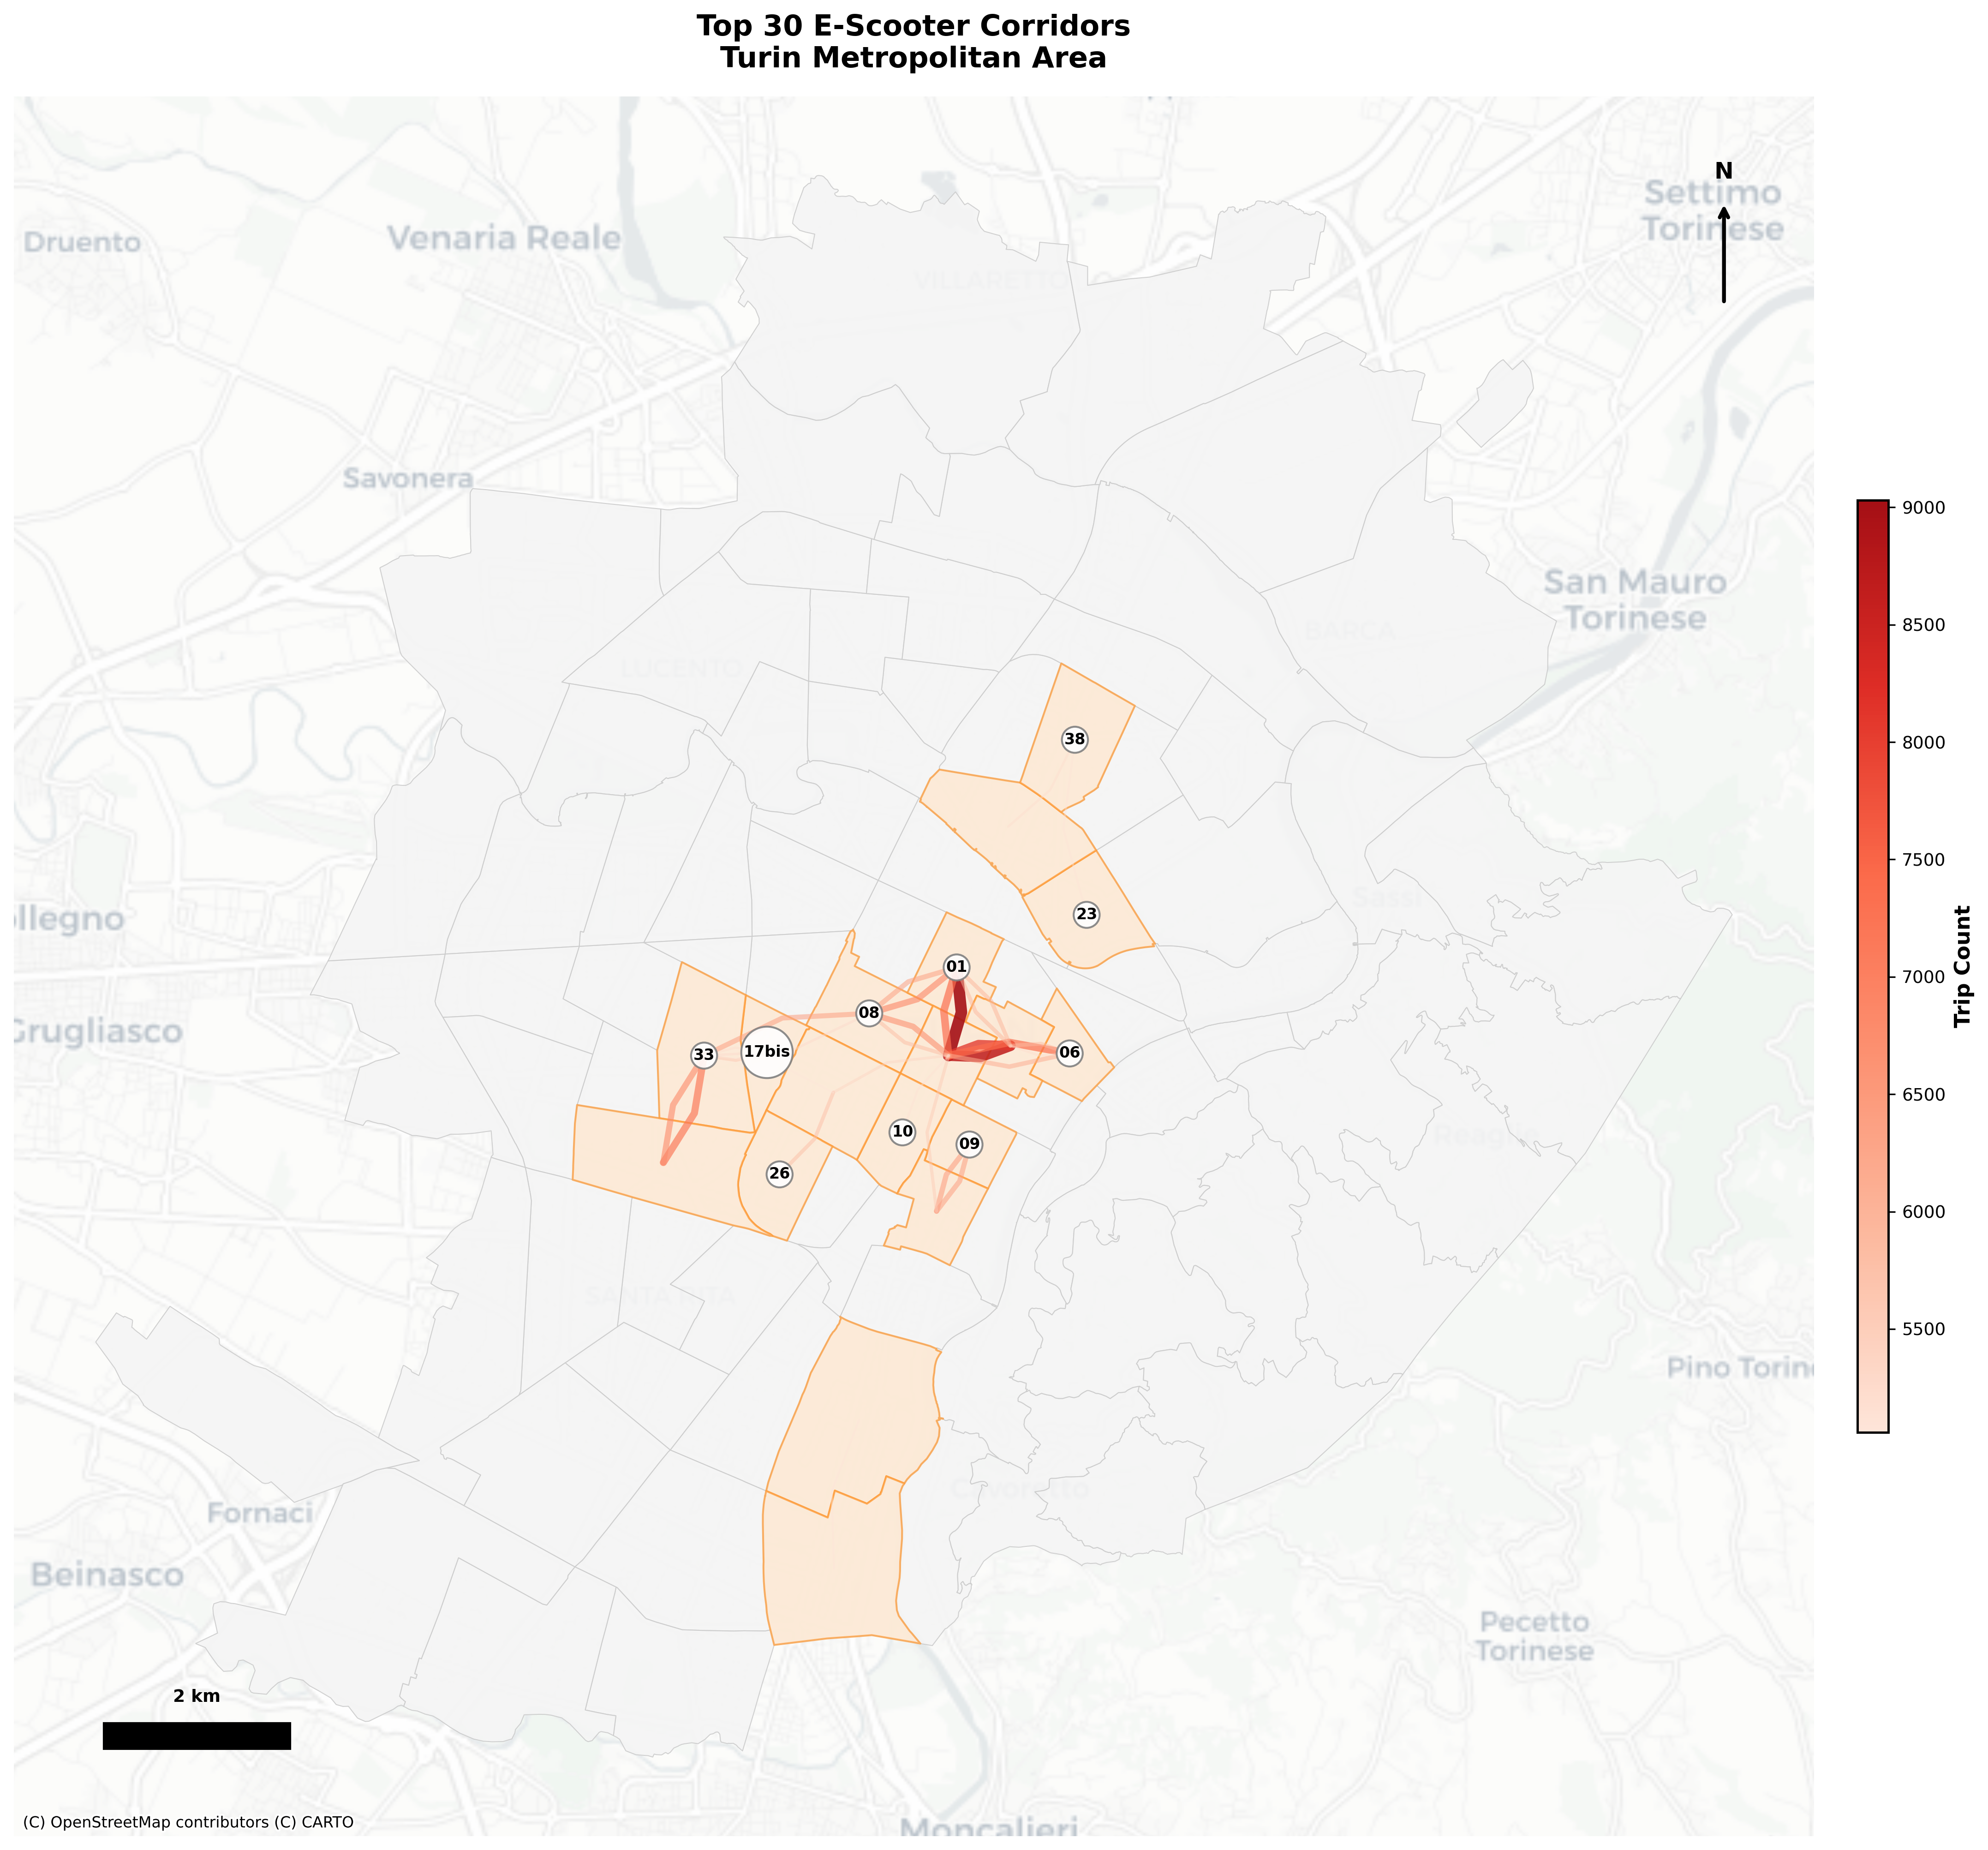
\includegraphics[width=0.95\textwidth]{figures/exercise2/spatial/flow_map_professional.png}
%     \caption{Spatial distribution of e-scooter flows in Turin, visualised using hierarchical clustering of zone-level origin-destination patterns.}
%     \label{fig:flow_map_professional}
% \end{figure}
